\chapter{Case Studies}
\label{results}
%do the usual introduction
% then explain wtf the idea is

In this Chapter, four scenarios are analyzed with the framework 
proposed in Chapter \ref{implementationall}.
In Section \ref{demandresponsesection}, a scenario
pertaining demand-response activities is studied.
In Section \ref{scenario2total}, a scenario
with an intended underconsumption of electricity is 
investigated. Then, in Section \ref{scenario3all},
a scenario with a sudden charging of electric vehicles
is analyzed.
In Section \ref{scenario4total}, a scenario 
based on a chemical accident where all entities act at 
the same time is studied.


\section{Scenario 1: Demand-Response Misinformation Campaign}
\label{demandresponsesection}

With the increased usage of information and communication 
technologies (ICT), new methods of influencing
consumer demand patterns are possible. 
These can be used by energy suppliers to influence the 
demand over time, e.g. to match energy consumption
with the energy generated by renewable energy sources such 
as solar panels. 
This concept of influencing the demand is called demand-response. 
With real time pricing (RTP), the electricity prices change
dynamically based on the total electricity demand.
The price changes are then forwarded to the customers with ICT, 
who are hence informed of the price changes.
The idea of RTP is that consumers change their electricity demand
by shifting activities with a high electricity usage, 
such as washing clothes or cooking, to time periods 
where the total electricity supply is higher and thus the prices
are lower.
RTP was already used in a variety of programs
under real life conditions \cite{barbose2004survey} 
and studies showed the benefits of such programs \cite{albadi2008summary}.

Rumors about changing prices spreading through social media may be of 
concern to utility companies.
In 2022, changes in the verification policies of Twitter allowed users 
to impersonate well-known brands such as Pepsi and Eli Lilly, leading to Twitter 
users being unable to determine which social media channels were
posting trustworthy information \cite{twitterchaos}. One user could
have used the policy changes of Twitter to impersonate	utility companies
and to advertise a false reduction of energy prices, leading to customers
believing the information and increasing their energy consumption as a 
reaction. Another possibility would be that hackers force access to the
social media profiles of utility companies and start sending false 
information to their customers. Hackers were already able to gain access
to the social media profiles of multinational companies in the past
\cite{twitterhacker}. Hackers could also spread misinformation in regards
to a false reduction in prices, thus leading to changes in consumer demand.

Thus, a possible scenario could be that hackers are able to 
access the social media profiles of a well-known utility company
to spread the information that the energy prices is reduced by 
a signifiant factor at a specific time. An example tweet is shown in 
Figure \ref{demandtweet}. This information is then  
spread around social media, reaching many customers of the energy supplier.

\begin{figure}[!ht]
    \center
    
\includegraphics[scale=.4]{figs/eondemandresponse.png}
    \caption{Example tweet that could be posted by hackers pretending to be an utility company}
    \label{demandtweet}
\end{figure}

\subsection{Estimation of Information Propagation Parameters}

To estimate the information propagation parameters for the scenario 
with the estimation 
algorithm, social media data is necessary. However, there seem to be 
no real examples of social media information propagation events 
which affected the power demand.
Thus, other information spreading events are used to estimate 
realistic model propagation parameters. The dataset used for this scenario
is the Typhoon Haiyan dataset \cite{david2016tweeting}. In this
dataset, $2.753.230$ twitter posts and their published dates were collected
to analyze user engagement on social media during a disaster. 
The twitter posts were collected
between November 8, 2013 and November 26, 2013. 
The propagation curve and the estimated infection curves can be seen in 
Figure \ref{propagationestimationtyphoon}. It can be observed 
that the parameter estimation algorithm models the infection progress
well, ignoring outliers such as the maximum value of the true information
propagation progress. Furthermore, the
information is assumed by the framework to have a high credibility 
of $\alpha=1$. The transmission rate is estimated to be
$\beta=0.65$.
Since the infection process is slow and progresses over 
multiple days, the verification parameter is
low with $p_{\mathrm{verify}}=0.001$. Last, the degree-to-node ratio
is also low with $\frac{k'}{N'}=0.006$.


\begin{figure}[!ht]
    \center
    \includegraphics[scale=.5]{figs/eval/scenario1/information.pdf}
    \caption{Information propagation progress for the Typhoon dataset 
    and estimated infection process}
    \label{propagationestimationtyphoon}
\end{figure}

\subsection{Simulation of the Scenario}

Multiple assumptions can be made to simulate the scenario.
First, it can be assumed that the time an entity receives the information
about the price reduction does not correlate with the time it will act on
it. Furthermore, since it is a widespread information propagation scenario,
a similar information propagation event can be used to analyze the 
results of the parameter estimation algorithm. Thus, the information propagation
parameters do not need to be defined. One work estimates 
the price elasticity of electricity in Germany to be $-0.4310$
\cite{priceelasticity}. 
This means that a price reduction of $1\%$
on the electricity price would lead to a $0.43\%$ increase in
electricity consumption. Hence, consumers 
respond well to such price reduction programs and it 
can be assumed that many people will act on the information.

Besides the estimated propagation parameters
the system parameters $p_{\mathrm{will\_act}}, p_{\mathrm{power\_usage}},
p_{\mathrm{available}}$ must be defined. Since the information 
propagated in the scenario
is believeable and it is assumed that customers respond well to price 
reduction programs, it can also be assumed that the two probabilities are 
reasonably high. For this simulation, values of $p_{\mathrm{will\_act}}=0.8$ and 
$p_{\mathrm{power\_usage}}=0.8$ were chosen. Furthermore, 
only one utility company is affected in this scenario and not the entire 
energy market. It is assumed that $50\%$ of the households of a city belong
to an utility company X, i.e. $p_{\mathrm{available}}=0.5$.
Since the information being spread in this scenario would both be 
well-received by the entities and since it is a believeable scenario, 
entities may also share the information with its neighbors even if they
cannot act on the information. A explanation as to why an entity cannot act 
on the information is that it is the customer of another utility company.
This scenario considers mostly energy-intensive household appliances.
The configuration file with all appliances considered in this
scenario can be found in the Appendix in Listing \ref{scenario1config}.

To evaluate this scenario, the simulation was run five times with five 
different seeds. In addition, a social media
graph model with $1000$ nodes is generated for the simulation. 
The simulation was run over $200$ iterations, with each
iteration $i$ being 15 minutes, resulting in a total time of $2$ days.
The results of the simulation can be seen in Figure \ref{firstscenariobasicresult}.
The left plot shows the power demand calculated by the model. The right 
plot shows the infection progress.


\begin{figure}[!ht]
    \center
    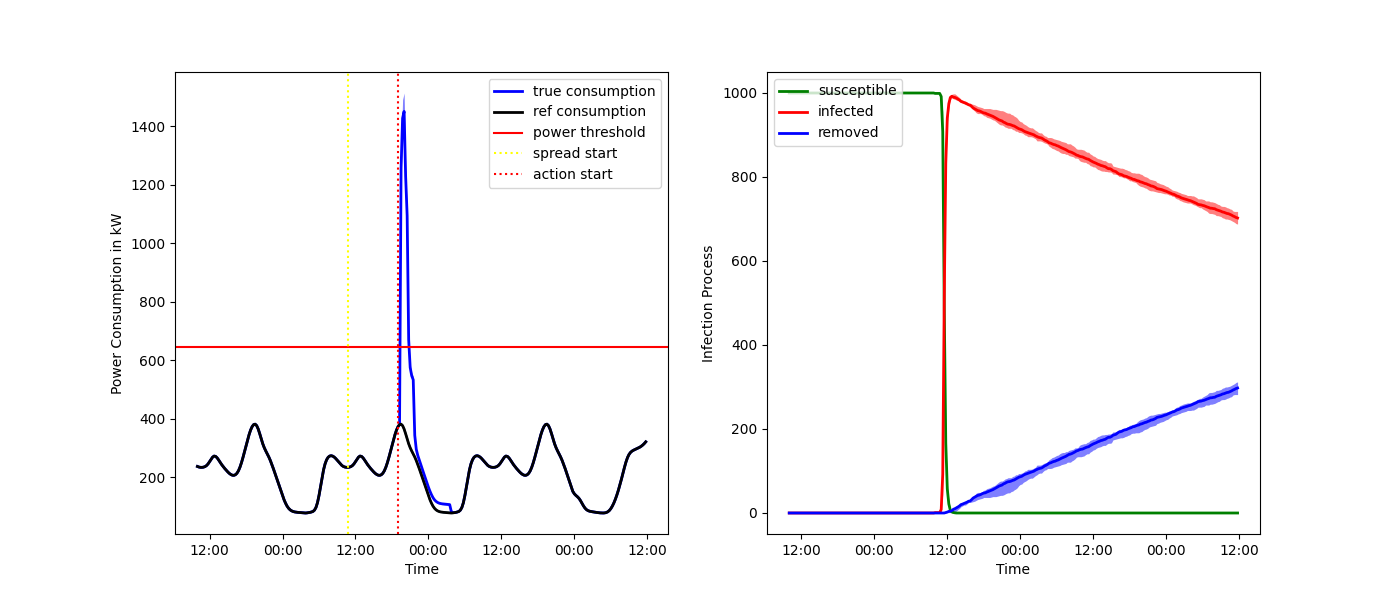
\includegraphics[scale=.5]{figs/eval/scenario1/basic_run.pdf}
    \caption{Simulation results for the first scenario. The lines in both plots show the average values over all simulations and 
    the lighter-colored areas around the lines show the minimum and maximum values
    over all simulations}
    \label{firstscenariobasicresult}
\end{figure}

For the power demand in Figure \ref{firstscenariobasicresult}, 
it is noticeable
that the power consumption spike generated by the infection is directly
after the time where entities can reasonably start acting on the information.
In addition, few hours after the spike, the excess power consumption
is reduced to an amount that is not critical for the power grid. 
The cause is that the time in which specific household appliances
such as dishwashers run are limited. Thus, after running a specific
appliance, it does not consume any more power. The result of the simulation
can be compared to the results of the simulation shown in 
Figure \ref{firstscenariobasicevchange}, where the duration of the 
appliance \textit{electric car} is changed from $32$ to $1000$ iterations.
In this Figure, it is noticeable 
that there is a constant overconsumption compared to the reference
power consumption shown with the black line since the electric car
does not finish using power.
In general, the 
results of the framework are robust and show little variance over the
different simulations. 

The infection progress in the right plot shows a rapid increase in infected 
individuals, followed by a slow, linear decrease in infected entities.
The rapid increase cannot be explained by the 
infection progress shown in Figure \ref{propagationestimationtyphoon}.
The Figure can only explain the slower decrease in infected entities. 
This mismatch between
the system-wide infection progress in Figure \ref{propagationestimationtyphoon}
and the infection progress generated by the graph-based algorithm 
in Figure \ref{firstscenariobasicresult} can have two reasons. 
First, the initialization assumptions of the simulation may be false.
In Section \ref{rulebasedpowerconsumption}, the simulation model
is defined with one node belonging to the \textit{Infected} class.
However, in Figure \ref{propagationestimationtyphoon}, it
is visible that the number of infected individuals at the 
time $t=0$ is more than one. This may lead to mismatches 
in the results. Second, the assumptions made in Section 
\ref{parameterestimationalgo} could be false. For example, 
the graph model is simplified such that the average number of 
neighbors belonging to a specific state $K$ is $k\cdot p^K(t)$, 
where $k$ is the average degree in the graph. However, nodes may 
have neighbors with significantly different state composition, 
especially at the beginning of the infection, based on where a specific 
node is in the graph and how close it is to the source of 
infection.

\begin{figure}[!ht]
    \center
    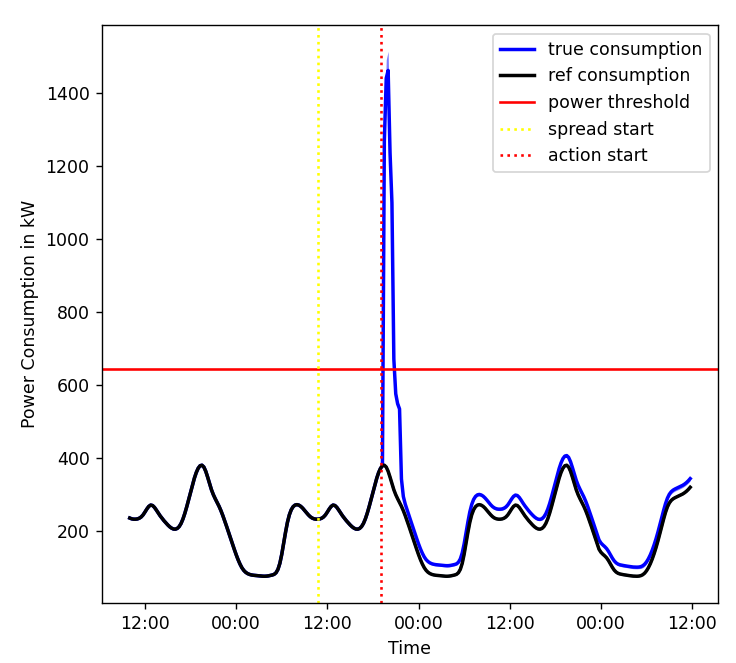
\includegraphics[scale=.6]{figs/eval/scenario1/longev.pdf}
    \caption{Simulation results for when increasing the duration to 
    charge electric cars to 1000}
    \label{firstscenariobasicevchange}
\end{figure}

\subsection{Analyzing the Information Propagation Model}

The propagation of information is a core concept of the simulation framework.
Hence, the sensitivity of the propagation process 
in regards to the parameters $\alpha, \beta, p_{\mathrm{verify}}$ 
should be analyzed. For the evaluation, the analyzed parameter was changed
while the other two parameters were fixed.
The fixed values for the parameters are 
$\alpha=0.4, \beta=0.2, p_{\mathrm{verify}}=0.2$. 
Both the infection progress and 
the immunization progress were analyzed.
The simulation was run five times with different seeds 
for each parameter value. The average of the simulation 
results are shown in the Figures \ref{scen1variablealpha},
\ref{scen1variablebeta} and \ref{scen1variablepverify}.


\begin{figure}[!ht]
    \centering
    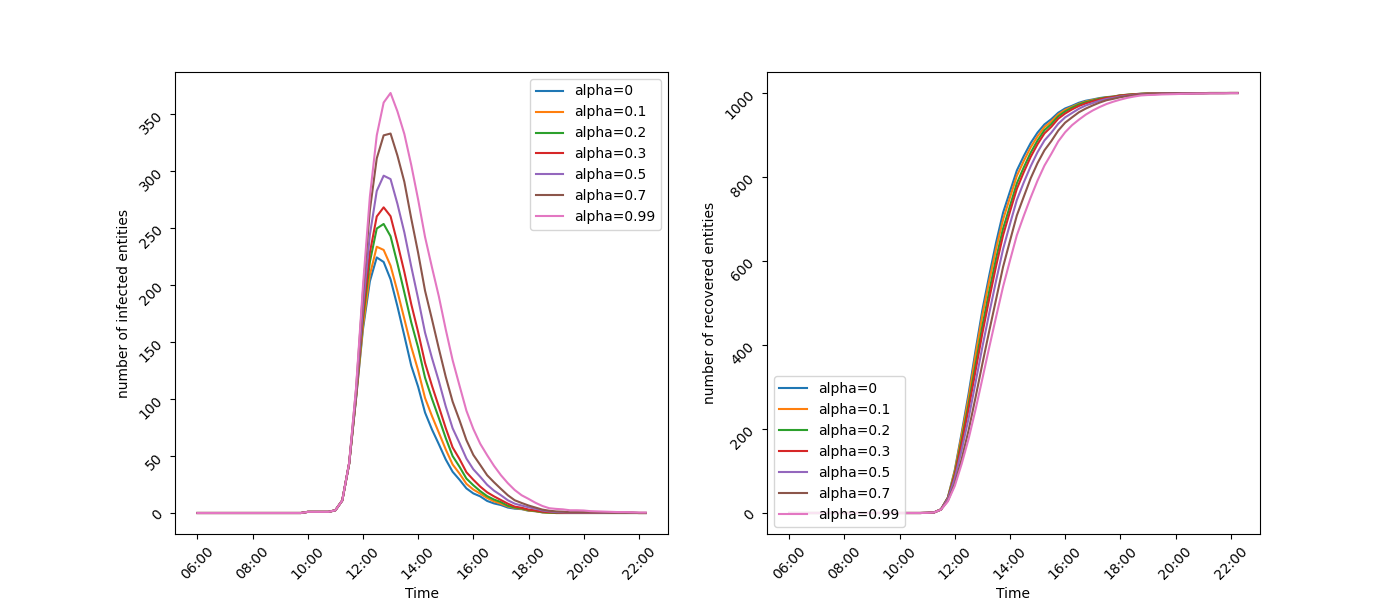
\includegraphics[scale=.5]{figs/eval/scenario1/alpha_mix.pdf}
    \caption{Infection process with changing variable $\alpha$}
    \label{scen1variablealpha} 
\end{figure}

\begin{figure}[!ht]
    \centering
    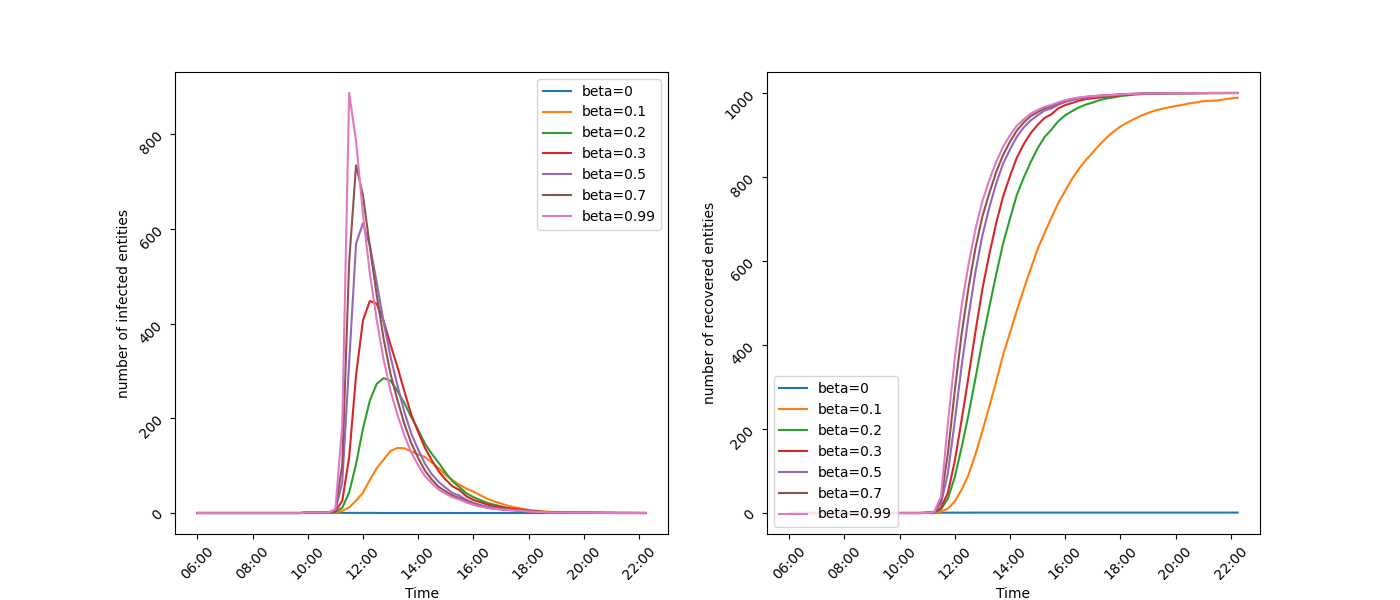
\includegraphics[scale=.5]{figs/eval/scenario1/beta_mix.pdf}
    \caption{Infection process with changing variable $\beta$}
    \label{scen1variablebeta} 
\end{figure}

\begin{figure}[!ht]
    \centering
    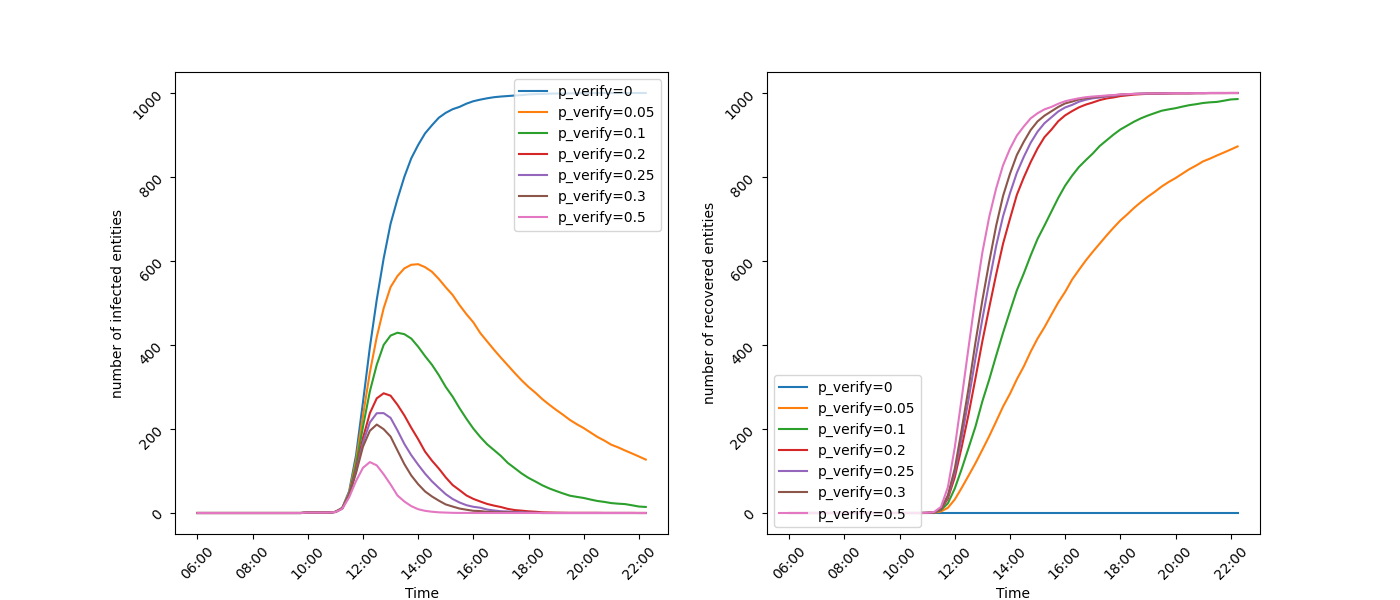
\includegraphics[scale=.5]{figs/eval/scenario1/verify_mix.pdf}
    \caption{Infection process with changing variable $p_{verify}$}
    \label{scen1variablepverify} 
\end{figure}

The infection process with
the verying parameter $\alpha$ is shown in Figure \ref{scen1variablealpha}. 
It is observable that with the given
parameters $\beta, p_{verify}$, the infection process is
not very sensitive to changes in $\alpha$, compared to changes 
in the other two parameters.
In Figure \ref{scen1variablebeta}, it is evident that the
infection process is more sensitive to changes in 
$\beta$ compared to $\alpha$. The maximum number of infected 
individuals increases with higher values for $\beta$.
The number of recovered individuals also increases with higher
$\beta$, suggesting that the system is more dynamic with higher 
$\beta$, increasing the speed that susceptible entities
become infected and later recover. Moreover,
the number of infected entities rises and falls at a greater rate with 
higher $\beta$. The propagation process is also 
sensitive to changes in $p_{verify}$, as shown in Figure \ref{scen1variablepverify}. 
The number of infected 
individuals reduce with higher $p_{verify}$, since a higher
number of entities can get informed with the true information
with higher $p_{verify}$ and can change their state to 
\textit{Removed}. As a consequence, the number of removed
entities increases faster with higher $p_{verify}$.
In general, it is visible that the number of infected
individuals increases quickly at the beginning of 
the simulation, independently from any
changes in the parameters $\alpha, \beta, p_{verify}$. 
The cause lies in the method to 
calculate the probability of the states of the entities.
At the beginning of the simulation, there are no recovered
entities, only susceptible and infected individuals.
Thus, considering Equation 
\ref{modified-SIS-table-equations}, it can be assumed
that the parameters $f_i, g_i$ have the values 
$f_i=\beta, g_i=0$ for a significant number of nodes
for the initial stages of the propagation process. 
Consequently, most nodes immediately 
change their state from \textit{Susceptible} 
to \textit{Infected} for a high value of $\beta$.
This means that the maximum number of infected 
individuals is reached in the early stages of the 
infection progress, followed by a slower decrease
in infected individuals. 

\subsection{Analyzing other Simulation Parameters}

Another set of parameters of interest for the evaluation
are the parameters which delay or prevent excessive
power consumption. These are the parameters $p_{\mathrm{power\_usage}},
p_{\mathrm{will\_act}}, p_{\mathrm{available}}$.
The sensitivity of the simulation results to these parameters
was tested by changing one of the parameters and leaving 
the other parameters fixed with the probabilities
$p_{\mathrm{power\_usage}}=1,
p_{\mathrm{will\_act}}=1, p_{\mathrm{available}}=1$.
The simulation was run five times with different seeds.
The simulated power usage values were substracted with the 
reference power 
usage values to show only the excessive power usage.

\begin{figure}[!ht]
    \centering
    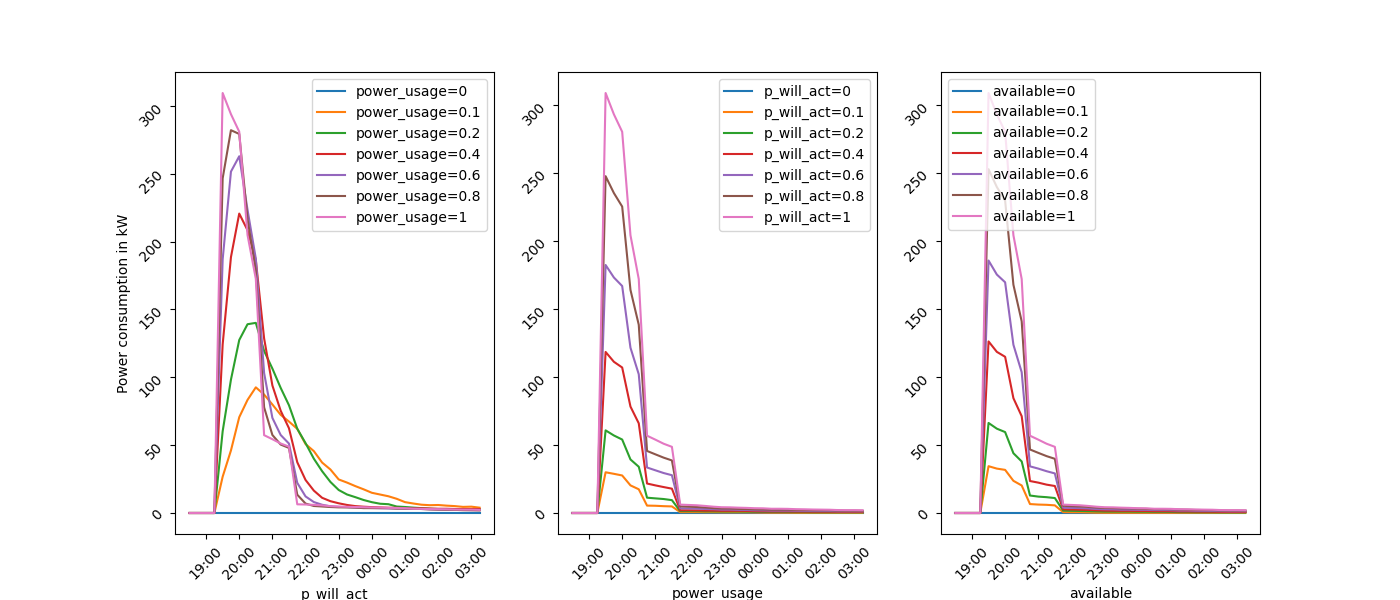
\includegraphics[scale=.5]{figs/eval/scenario1/powervars.pdf}
    \caption{Excess power usage curve with different 
    $p_{\mathrm{power\_usage}}, p_{\mathrm{will\_act}}, 
    p_{\mathrm{available}}$}
    \label{scen1variablepowervals} 
\end{figure}

The average values of the simulation results are shown in 
Figure \ref{scen1variablepowervals}. The Figure shows that
the excess power usage calculation 
is very sensitive to changes in all
three parameters. If any of the parameters is $0$, no
excess power consumption occurs. The reason is that 
for an entity to consume more power, it needs to fullfill
all conditions which are related to the three 
probabilities. If one of the probabilities is $0$, 
no entity can fulfill the condition related to the 
specific probability. Moreover, with increasing parameter
values, the excess power consumption increases. The 
cause is that with higher probabilities, it is 
easier for the entities to fulfill the condition
related to the specific probability. As a 
consequence, more entities consume more 
power and the total excess power demand increases.
In addition, it can be seen that the excess power 
demand progress is slower for the parameter 
$p_{\mathrm{power\_usage}}$ than for the other parameters.
The reason is that the parameter delays the 
excess power consumption, it does not prevent it.
Therefore, fewer entities consume excess energy at the 
same time. As a consequence, 
a low value for $p_{\mathrm{power\_usage}}$
stretches the power consumption curve, leading
to a less critical, but longer lasting 
overconsumption period. This can also be seen in Figure 
\ref{scen1variablepowerusage}, where lower 
$p_{\mathrm{power\_usage}}$ leads to 
a longer overconsumption period with a lower peak demand.


\begin{figure}[!ht]
    \centering
    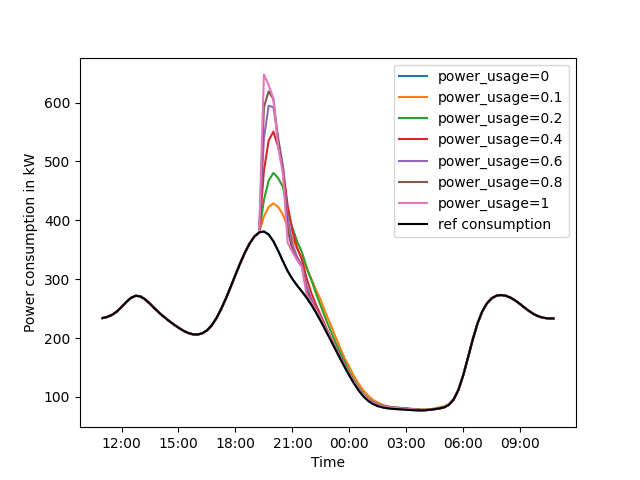
\includegraphics[scale=.6]{figs/eval/scenario1/powerusage.pdf}
    \caption{Excess power usage curve with different values for 
    $p_{\mathrm{power\_usage}}$}
    \label{scen1variablepowerusage} 
\end{figure}

\section{Scenario 2: Coordinated Action of Extremists 
against the Electrical Grid}
\label{scenario2total}
So-called echo chambers on various social media websites allow people to 
hear biased opinions and news which confirm their views on 
various topics \cite{terren2021echo}. This leads to political
polarization and extremism \cite{van2022banality}.
These people may consequently try to fight the established political
system. Research shows that social media can influence people
to commit hate crimes \cite{muller2021fanning}.
In general, the number of violent incidents caused by
extremists, specially right-wing extremists, is rising 
\cite{koehler2016right}. 
Most of the criminal acts caused by political extremism 
in Germany are in the fields of property damage, 
propaganda crimes, insults and hate speech \cite{bmicrimestatistics}.
However, extremists also cause more serious crimes. In 2022,
right-wing extremists planned to sabotage the electrical grid 
infrastructure by destroying power lines \cite{anschlagstrom}.
Thus, critical infrastructure may be a target
for political extremists. 

An additional way to target critical infrastructure is with coordinated
actions from many entities. The intention may not necessarily be harmful. 
For example, during Earth day, people were encouraged to switch off their 
lights and appliances at a specific day to save energy \cite{earthday}.
However, extremists could also synchronize their actions to reduce their
power consumption to a minimum, thus mismatching electricity supply
and demand by a considerable degree. Utility companies would 
hence need to deal with a sudden mismatch of supply and demand in 
the power grid.

Thus, a possible scenario could be 
that extremists plan to turn off all their electrical devices at 
a specific time to destabilize the system. The
time would be announced in advance. An example message spread by
these extremists can be seen in Figure \ref{schwurbler}.

\begin{figure}[!ht]
    \center
    
\includegraphics[scale=.7]{figs/schwurblerchat.png}
    \caption{Example message that could be posted by extremists on Telegram}
    \label{schwurbler}
\end{figure}

\subsection{Simulation of the Scenario}
 
Multiple assumptions can be drawn for the scenario.
First, it is assumed that the time when an entity receives the
information does not coincidences with the time when it acts on the information.
Furthermore, it is unlikely that large parts of the population wil
act on the information in this scenario 
since it is assumed that only a small minority
of the population will act on extremist ideologies. But the
entities that are open for such ideas are likely to act on the 
messages that they receive.
This means that the parameter $p_{\mathrm{available}}$ has a low value,
whereas $p_{\mathrm{power\_usage}}, p_{\mathrm{will\_act}}$
have high values. For this scenario, the values 
$p_{\mathrm{available}}=0.2, 
p_{\mathrm{power\_usage}}=1, p_{\mathrm{will\_act}}=1$
were chosen.
Moreover, it is expected that infected individuals will not 
believe in any information that goes against the original message.
Therefore, it is assumed that $p_{\mathrm{verify}}=0$. Next, it
can be considered that the information is believable to 
the affected population and that it is quickly spread by 
the infected entities, i.e. it is assumed that $\alpha=1, \beta=1$.
However, the information is not believeable to the people 
who are not open to extremist messages. This means 
that entities that are not receptive to the messages, 
do not forward the information to other entities.
Next, it is assumed that all infected entities 
stop consuming power. Thus,
the power usage factor $a$ is set to zero.
The configuration file for the framework can be viewed in the Appendix in
Listing \ref{scenario2config}.

To analyze the scenario, the simulation was run with five 
different seeds. Furthermore, a model with $1000$ nodes was used 
for the evaluation. 
The simulation was run over $200$ iterations, with each
iteration $i$ being 15 minutes.
The number of infected individuals 
is not high, as observed in Figure \ref{schwurblerresults}.
Only 200 of 1000 nodes get infected. The reason is 
that $p_{\mathrm{available}}=0.2$, therefore only $20\%$ of the nodes
can get infected. In addition, it is visible that the results 
are not very robust because the results change heavily in different 
simulations. The reason is that depending on the network structure
and which entities can get infected and will act on the information, 
the infected entities may not be able to infect all other entities
that could get infected. Entities that can get infected may be 
connected to entities that are not susceptible to the conspiracy 
theory and do also not forward the message to other entities
open to the conspiracy theory, hence limiting the 
spread of misinformation.
Moreover, it can be seen that of underconsumption
is higher in peak load periods compared to periods with 
lower load. This is reasonable since infected households would 
normally use more energy during peak load times. Their absence
means that a higher amount of power demand is missing 
during these periods. Additionally, the decrease in demand 
changes immediately at the moment where the entities 
could change their action. This means that the changes 
in power demand are abrupt and could surprise the responsible 
power suppliers.

\begin{figure}[!ht]
    \center
    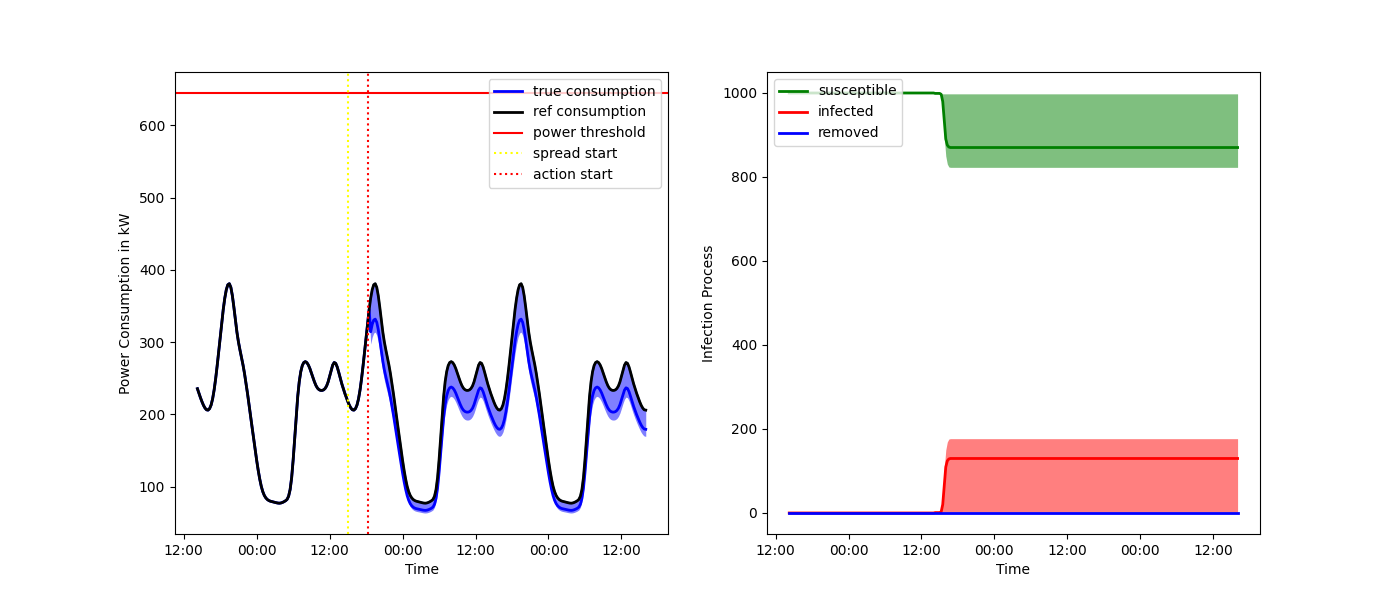
\includegraphics[scale=.55]{figs/eval/scenario2/basicplot.pdf}
    \caption{Simulation results for the second scenario}
    \label{schwurblerresults}
\end{figure}

\begin{figure}[!ht]
    \center
    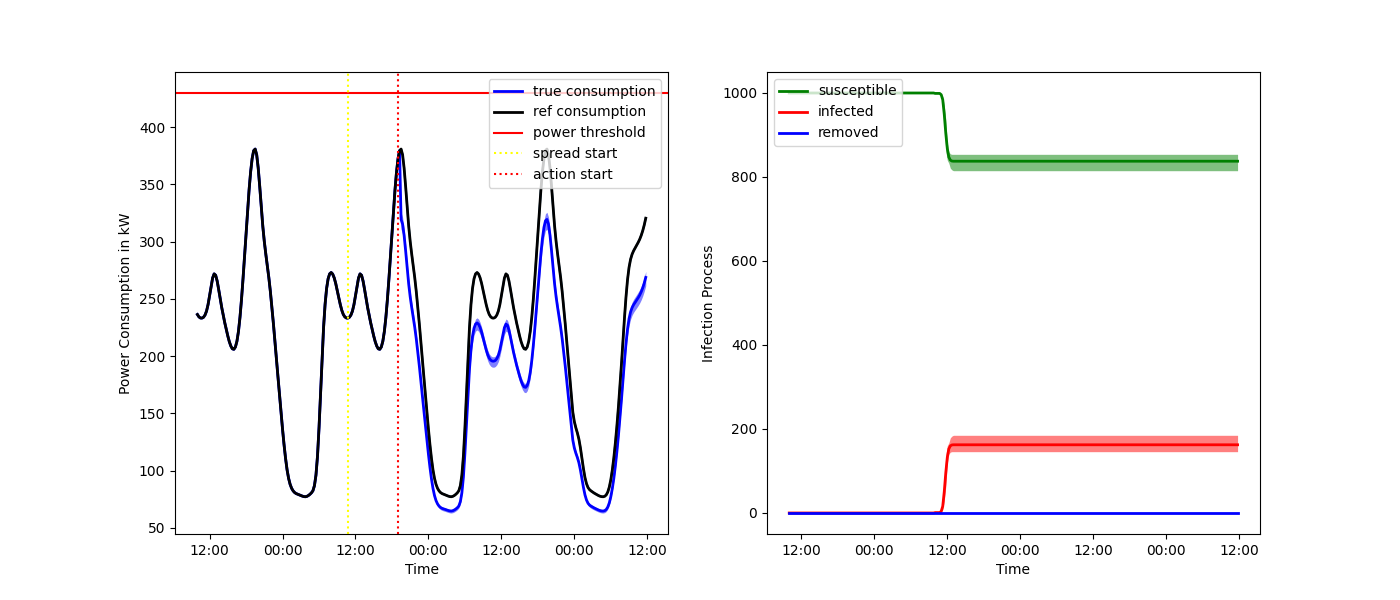
\includegraphics[scale=.55]{figs/eval/scenario2/fringeoff.pdf}
    \caption{Simulation results when all nodes forward the information}
    \label{schwurblerresults2}
\end{figure}

In Figure \ref{schwurblerresults}, it can be seen that 
the results of the simulation are not robust. To analyze the 
robustness of the simulation in regards to the message 
forwarding, the simulation is changed so that all entities
forward the information, even if they do not act on the information. 
The simulation was run five times with five different seeds. 
The simulation results in Figure \ref{schwurblerresults2} show 
that if all entities forward 
the information, the simulation results are more robust. 
The reason is that if not all entities forward the messages,
the infection process may be hindered and thus not
all nodes can get infected. The concept of non-believing entities
not forwarding messages
was implemented by creating nodes which are not available and thus
do not use additional power consumption
also not able to forward the information to other nodes.
These nodes can hinder the information propagation process.
However, this idea may not be realistic. Smaller communities,
such as extremist communities, may 
be tightly connected. Therefore, there may be no information 
barriers that could hinder the flow of information between 
entities that are open for this kind of information.


\section{Scenario 3: Mass Evacuation of a City due to a Disaster}
\label{scenario3all}

Sometimes the dangers in a disaster are so severe that 
authorities choose to order the evacuation of the affected population.
For these types of evacuation, the autorities may use emergency channels 
to inform the population of the evacuation.
However, people may also choose to leave the city in masses on their own accord.
The information of a possible disaster, such as a wildfire, reaching the
city soon or other disasters may be spread through social media and 
lead to fear in the population. As a consequence, people may 
want to leave the possibly affected region to reach a safe location.
If people decide to leave their homes to flee from the disaster, many
will probably use their cars as the mode of transportation.
The increased adoption of electric vehicles (EV)
leads to people needing to recharge their EVs if they wish 
to drive them. An evacuation could lead to many people charging
their cars at the same time, thus increasing the power demand 
to a level which is critical for the power grid. 

Hence, a possible scenario could be that 
rumors about a wildfire spreading towards a city leads to people
trying to leave the city in masses. In addition, a significant 
number of people drive EVs, thus giving them the need to charge
their cars before they are able to leave the city. An example
tweet spreading the rumor is depicted in Figure \ref{firetweet}.

\begin{figure}[!ht]
    \center
    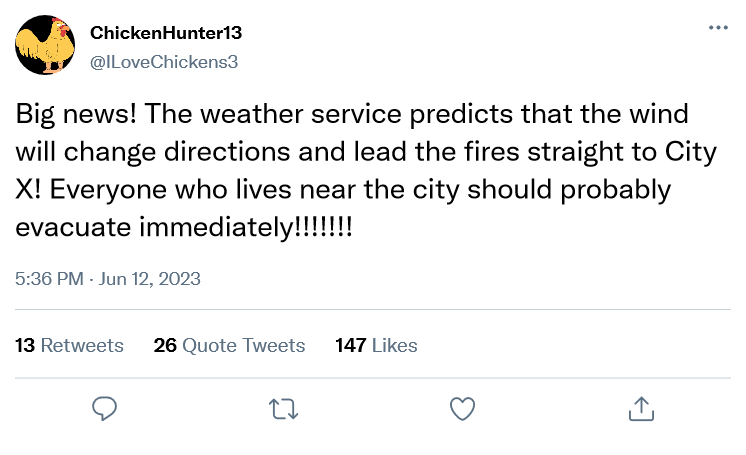
\includegraphics[scale=.4]{figs/firenews.png}
    \caption{Example tweet that could posted by an anonymus user on Twitter}
    \label{firetweet}
\end{figure}

\subsection{Estimation of Information Propagation Parameters}

This scenario uses social media data to estimate the information 
propagation parameters.
The parameters were calculated with 
the estimation algorithm 
presented in Section \ref{parameterestimationalgo}. 
For the estimation, a 
twitter dataset was used.
The data contains $22787$ Tweets posted during December 4 2020.
The results of the estimation framework can be seen in 
Figure \ref{geoloctweet}. Figure \ref{geoloctweet} shows 
that the dataset contains the start of a 
information propagation process.
Thus, this dataset can be used as an example dataset 
to show how the excess power consumption progress 
could be analyzed at the beginning of an infection.
The estimated infection progress show that the number of infected
individuals rises monotonously. Furthermore, the infected 
entities do not change their state to \textit{Removed}.
The parameters estimated by the framework are 
$p_{verify}= 0.0, \alpha = 0.8, \beta = 0.56$.
Moreover, the estimated social media graph is 
connected more tightly compared to the 
scenario described in Section \ref{demandresponsesection} 
with the node degree ratio being 
$\frac{k'}{N'}=0.53$. 

\begin{figure}[!ht]
    \center
    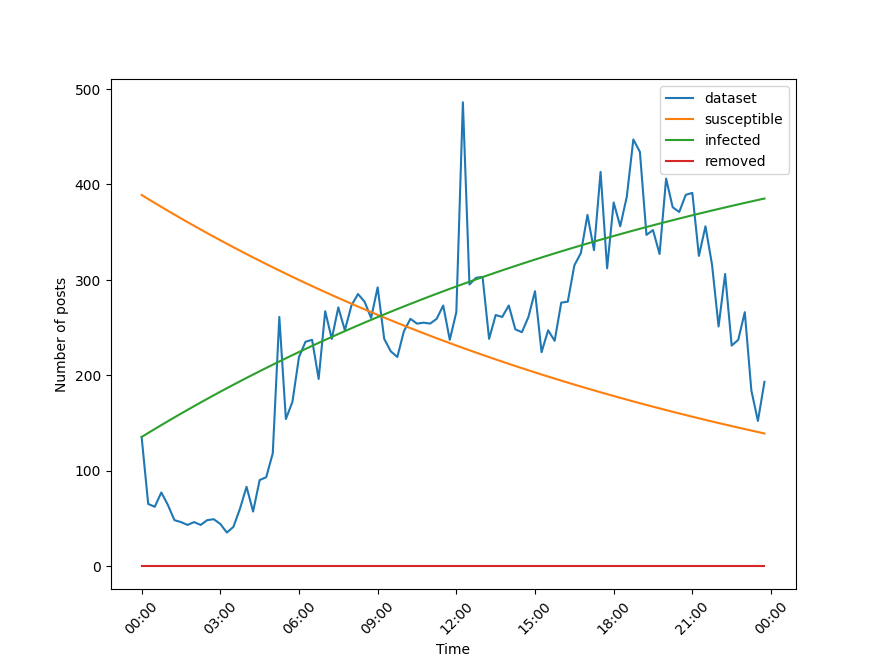
\includegraphics[scale=.6]{figs/eval/scenario3/informationpropagation.pdf}
    \caption{Information propagation progress for the soccer dataset 
    and estimated infection process}
    \label{geoloctweet}
\end{figure}

\subsection{Simulation of the Scenario}

Multiple assumptions can be drawn to define the simulation parameters. 
In 2023, $2.1\%$ of all cars in Germany were 
EVs \cite{evadoption}. Thus, $2.1\%$ of all households in the simulation
possess an EV. Moreover, it is assumed that 
each 15 minutes, $1.75$kWh is used to charge the EV 
and that most people stop charging after one hour
to leave their residences and flee from the city with their EVs.
Due to the severity of the rumor,
all people are assumed to act immediately upon 
receiving the information. Therefore, it is assumed 
that $p_{\mathrm{available}}=1, 
p_{\mathrm{power\_usage}}=1, p_{\mathrm{will\_act}}=1$.


The simulation was run five times with five different seeds. 
A social media graph with $1000$ nodes was used for the simulation. 
The simulation was run over $200$ iterations, with each
iteration $i$ being 15 minutes.
The excess power consumption created in this scenario is negligible, 
as observed in Figure \ref{thirdscenarioresults}.  Hence, the 
synchronized charging of the given amount of EVs does not
lead to significant spikes in power usage.
The reason is that the current adoption rate of $3\%$ is low.

\begin{figure}[!ht]
    \center
    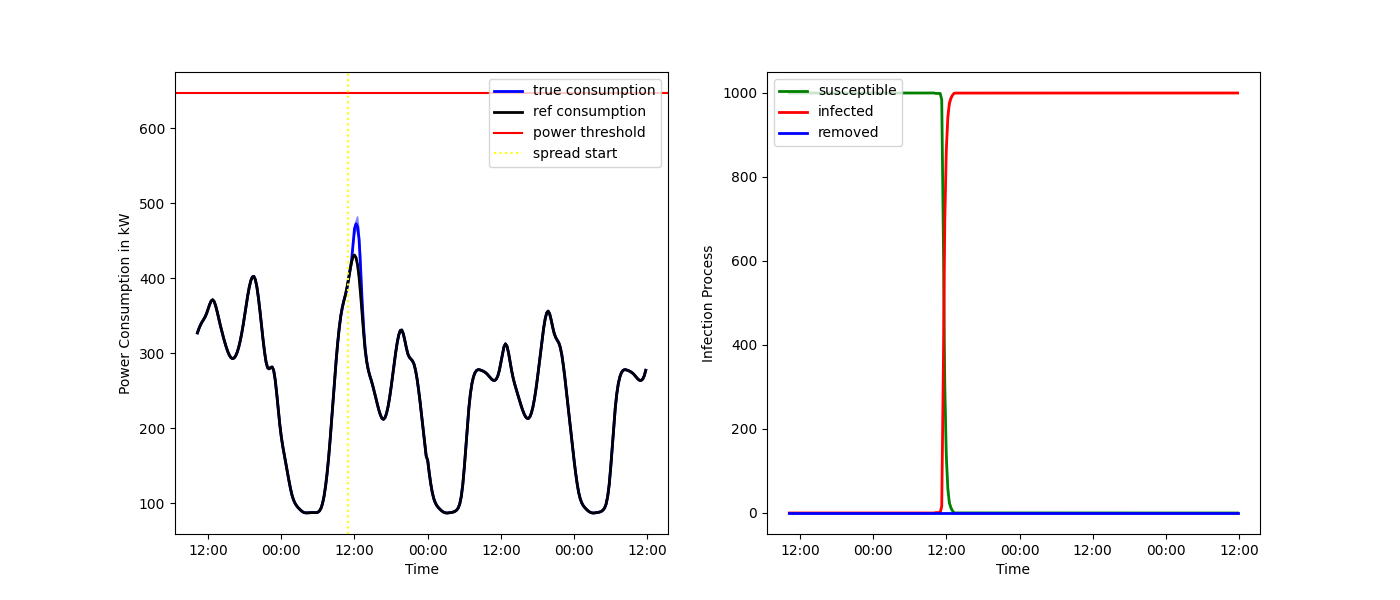
\includegraphics[scale=.5]{figs/eval/scenario3/scenario3basic.png}
    \caption{Simulation results for the third scenario}
    \label{thirdscenarioresults}
\end{figure}

However, with the increasing adoption of EVs in the 
population, the danger of synchronized charging 
of EVs increases. In Figure \ref{thirdscenarioresultsdiffadoption},
it can be observed that with increasing adoption of EVs,
the power usage spikes created by syncronized charging 
increases significantly. In the simulation framework,
an adoption rate of $20\%$ is enough to create a 
blackout given the critical threshold 
defined in the simulation.

\begin{figure}[!ht]
    \center
    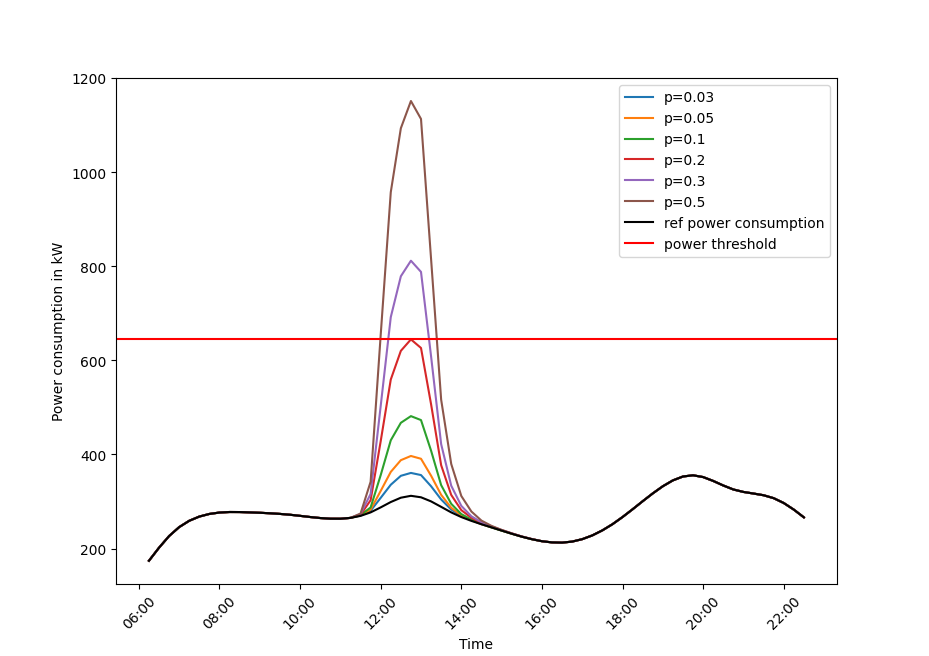
\includegraphics[scale=.5]{figs/eval/scenario3/changingadoption.png}
    \caption{Simulation results with different adoption rates for EVs}
    \label{thirdscenarioresultsdiffadoption}
\end{figure}

\section{Scenario 4: Mass Showering after a Chemical Accident}
\label{scenario4total}

With the increasing usage of ICTs in the population,
new methods to inform people about extreme circumstances
such as natural disasters or other catastrophes are possible. In 2022,
a new warning system called Cell Broadcast was introduced in Germany
\cite{TEAlert}. Cell Broadcast can be used to warn the population
of emergencies by sending all cellphone users in the 
region of interest a message with an alert tone.
Furthermore, with the growing threat of climate change, many countries
are adopting measures to reduce the societal impact on the
climate. One of the fields that these measures affect 
are heating technologies. Currently, $75\%$ of the households 
in Germany heat with fossil fuels \cite{bdewhouhseholds}. 
However, there are measures being 
implemented to increase the usage of renewable resources such 
as electricity from solar panels in residential heating
\cite{heizungsgesetz}. Therefore, the number of households 
using electricity for heating are increasing, with 
$57\%$ of newly build houses installing 
heat pumps, which use electricity to heat
\cite{heatingpumps}.

Germany has one of the biggest chemical industry sectors in the world.
It is home to big chemical factories in cities such as Ludwigshafen and
Darmstadt. Areas with chemical factories have the risk of being
affected by chemical accidents.

A possible scenario is that a chemical accident in a 
factory near a major city leads to dangerous chemicals 
leaking out. These chemicals spread through the air 
and adhere to the skin of humans, leading to serious 
health problems if they stay on the skin for too long.
Thus, the city's government uses Cell Broadcast to
instruct the population to close their windows and 
to take a shower to remove the chemicals from their bodies.
Hence, most people shower at the same time,
using electric heat pumps to heat up their water to shower.
An example message can be seen in Figure \ref{warningmessage}.

\begin{figure}[!ht]
    \center
    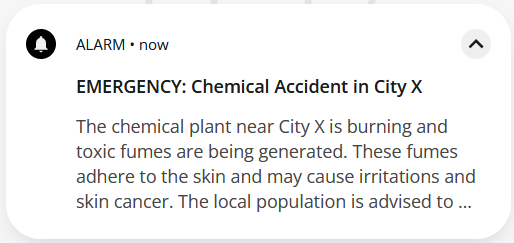
\includegraphics[scale=.7]{figs/emergencychemical.png}
    \caption{Example warning message that could be received via Cell Broadcast}
    \label{warningmessage}
\end{figure}

Given the scenario description, multiple assumptions can be
made for the simulation.
First, it is assumed that since Cell Broadcast is used, the simulation
will reach all entities in the city at the same time.
Furthermore, since the information comes from a verified channel,
all entities will believe the information. In addition, the time where the
entities receive the information is also the time where they will act
on it.
Moreover, since this scenario is a synchronous event, it can be 
assumed that the
maximum number of infected individuals at the same time equals
the total number of entities in the system, thus $I(t_{max})=N$.
Consequently, the usage of the simulation framework is not necessary
and the results of this scenario can be calculated manually.
Darmstadt is chosen as the example city for this scenario analysis.

\subsection{Analytical Calculation of the Scenario Results}

Darmstadt is a city with $89194$ households by 2020 
\cite{statistadarmstadt}. The BDEW
says that $3\%$ of the households in Germany currently use
heat pumps for heating. Therefore, it can be assumed that 
$0.03 \cdot 89194 \approx 2675$ households currently use 
heat pumps. An average heat pump uses about $2$ kWh per hour, 
or $0.5$ kWh per 15 minutes.

If it is assumed that all households in Darmstadt receive 
a message at the same time via Cell Broadcast and that
every household takes a hot shower for 15 minutes,
there will be an additional 
demand of $0.5\,kWh \cdot 2675 = 1337.5\,kWh $ for these 
15 minutes. If an average household uses $3900\,kWh$ 
per year and $0.45\,kWh$ per hour, then using the heat pump 
would double their average power consumption for a short time.

\subsection{Calculation of the Scenario Results with the Simulation Framework}
To check if the simulation framework calculates the same 
results, the framework was configured with immediate
propagation of information. Thus, the propagation
parameters is set as 
$\alpha=1, \beta=1, p_{verify}=0$. 
Furthermore, it is assumed that all infected 
individuals will immediately act on the information.
Therefore, the activation parameters are 
set as $p_{\mathrm{available}}=1, 
p_{\mathrm{power\_usage}}=1, p_{\mathrm{will\_act}}=1$.
In addition, the duration of the heat pump is set to one iteration.
The configuration file is provided in the Appendix in
Listing \ref{scenario4config}.

The simulation was run five times with five different seeds. 
Furthermore, since the simulation framework is unable
to handle models that are too big, a graph model with 
$892$ nodes was used for the evaluation. 
The results of the simulation can be seen in 
Figure \ref{warningmessagesimulations}.
In the Figure, it is visible that the excess power 
consumption is similar to the calculated excess
consumption. Since the model size is approximately
$\frac{1}{100}$ of the size of Darmstadt, the 
excess power consumption should be
$1337.5\,kWh\cdot \frac{1}{100} \approx 13.3\,kWh $.
However, the excess power consumption 
calculated by the simulation is $12\,kWh$.
Thus, it is lower than the analytical result.
The reason is that given the implementation of the 
framework, not all nodes can be infected at the first
iteration step $t_0$. This can be observed in the 
left plot in the Figure. The function showing the 
number of infected entities does not immediately
rise to the number of all entities in the system.
Given the propagation 
parameters, for each iteration step $t_{i}$ all
neighboring nodes of all infected nodes that
are not infected become infected. Thus, for 
all nodes to become infected, $j$ iteration steps 
are needed, where $j$ is the least number of hops between 
the initial source of infection and the furthest 
node. Since the additional usage of the heat pump 
lasts one iteration step, the excess power usage
of the heat pump is distributed over 
the timespan $[t_0, t_j]$. 
This means that the 
usage of the heat pumps is not fully synchronized.
Therefore, the simulation framework is unable
to simulate scenarios where all entities 
are informed and thus become infected at the 
same time. 


\begin{figure}[!ht]
    \center
    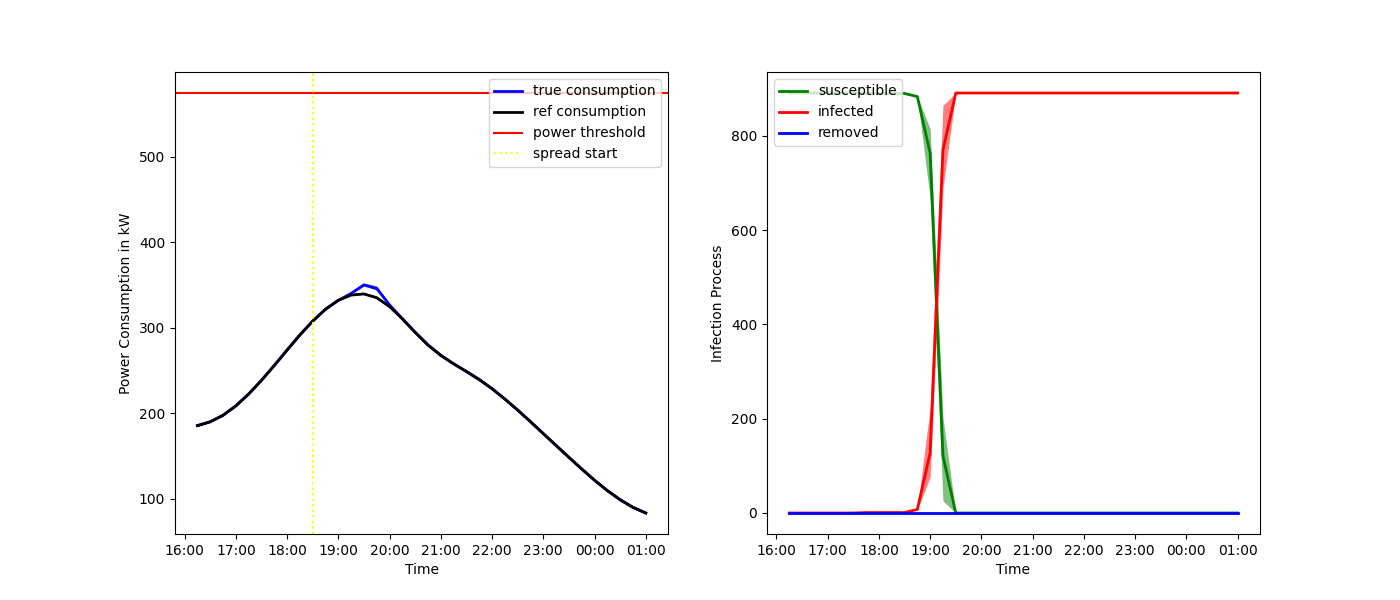
\includegraphics[scale=.53]{figs/eval/scenario4/basic_plot.pdf}
    \caption{Simulation results for the chemical accident scenario}
    \label{warningmessagesimulations}
\end{figure}

As a conclusion, the duration of the appliance 
usage may affect the results of a scenario where 
all entities receive the information at the same time.
However, if the number of hops $j$ is smaller than
the minumum duration of the relevant appliances $d$,
then the maximum excess power consumption should 
be the same as the analytical result. 
In Figure \ref{warningmessagedifferentdurations},
the maximum excess power consumption was calculated
for different durations $d$ for the heat pump.
It can be observed that the maximum excess power 
consumption increases with the duration $d$.
At duration $d=4$ iterations, the maximum excess power consumption
increases from $12kWh$ from duration $1$ to 
$12.7kWh$. Thus, with a longer duration $d$, the 
analytical results can be approximated.
Last, in Figure \ref{warningmessagedifferentadoptionrates},
it is visible that with increasing number of households 
that use heat pumps, the maximum excess power consumption
increases.

\begin{figure}[!ht]
    \center
    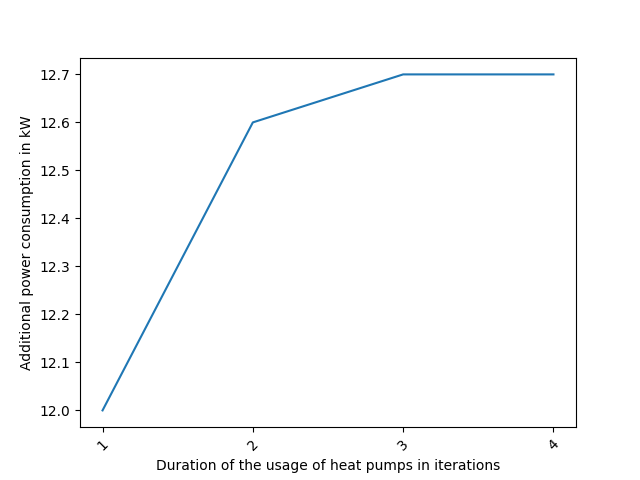
\includegraphics[scale=.7]{figs/eval/scenario4/durationeval.pdf}
    \caption{Excess power consumption given different durations}
    \label{warningmessagedifferentdurations}
\end{figure}


\begin{figure}[!ht]
    \center
    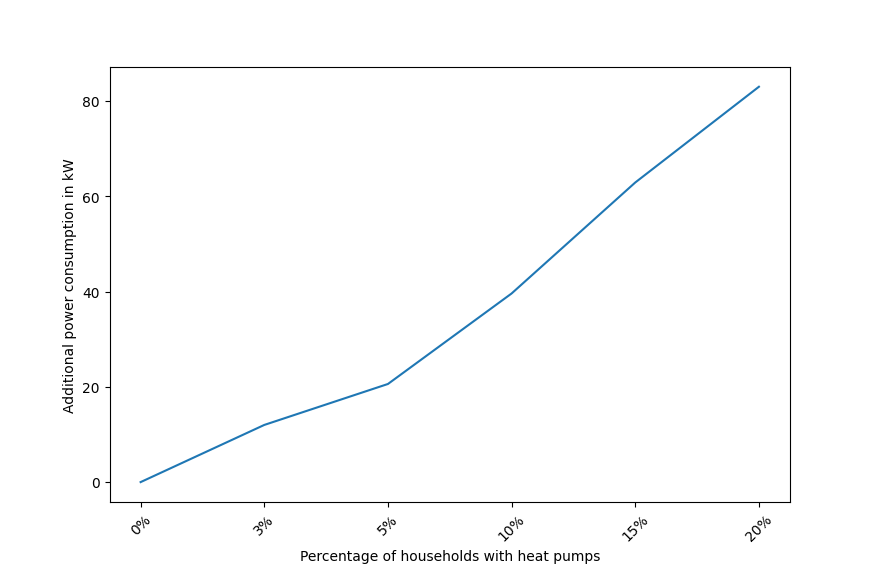
\includegraphics[scale=.6]{figs/eval/scenario4/percentageeval.pdf}
    \caption{Excess power consumption given different adoption 
    rates for heat pumps}
    \label{warningmessagedifferentadoptionrates}
\end{figure}

